
\chapter{Generative Modelling}

\section{Variational Autoencoders}

Variational Autoencoders (VAEs) are one of the most commonly used and efficient approaches for the task of generative modelling. Unlike discriminative models, whose objective is to learn the conditional distribution of the data $\underbar{x} = x_1, \dots, x_n$, i.e. estimate $p(x)$ with the parametri distribution $p(x,\theta)$, typically differentiable with respect to $\theta$. 

In this way, it becomes possible to sample from such a probability distribution, thus generating new instances similar to the training dataset, or to assign to a given instance the probability of having been generated by the same process as the training dataset.

In general, generative modelling deals with a harder task with respect to discriminative models because in the former there is much more knowledge to learn. Intuitively, this is valid also for humans: by seeing many labelled images of dogs and cats it is much easier to distinguish dogs from cats than to draw a new image of a dog and a cat. In fact, in order to assign a label it is only required to find out some patterns which are different between the categories, while to generate a new instance it is necessary to capture correlations in the dataset, as for example the fact that dogs have two eyes, a tail, etc.. So, the discriminative model has to learn a decision boundary in the data space, while the generative one has to understand how data is planced throughout the space. 

\begin{figure}[H]
    \centering
    \includegraphics[width=0.8\textwidth]{assets/fig45.png}
    \caption{Image from \textit{https://medium.com/@jordi299/about-generative-and-discriminative-models-d8958b67ad32}}
    \label{fig:vae}
\end{figure}

It may be more convenient to avoid learning directly the distribution of the data (pixels in our example), but to introduce latent features $z$ which can describe the data and rewrite our distribution as 

$$
p(x,z|\theta) = p(x|z,\theta)p(z)
$$

We assume that the posterior distribution $p(z|x)$ is intractable and that we are working in the big data regime, so that we are forced to consider mini-batches during the training phase. The goal that we would like to achieve are:
\begin{itemize}[label=$\blacktriangleright$, leftmargin=2em, itemindent=0em]
    \item Learning the parameters $\theta$
    \item Approximating the posterior $p(z|x)$ in order to understand which are the latent features extracted from a given instance $x$
    \item Performing approximate inference on $x$ to be able to fill holes in an instance 
\end{itemize}

In this scenario, where we have a parametric distribution with latent variables, it might occur to use to use Expectation Maximization. But we must remember that the E-step requires being able to evaluate the conditional distribution $p(z|x,\theta_{OLD})$ which we have assumed here to be intractable. Other techniques that we have already seen, such as mean field variational approximation or sampling-based methods, turn out to be too computationally expensive as they do not scale well with large datasets. We will now see how to solve the problem by applying stochastic variational inference together with an encoder-decoder approach.

\subsection*{Autoencoding Variatinoal Bayes (AEVB)}

Following the idea of black-box variational inference, we start by considering a parametric variational distribution for the latent variables $q(z|\phi)$. We would like to optimize the ELBO jointly on $\theta$ and $\phi$ by stochastic gradient ascent and so we need to compute $\nabla_{\theta,\phi}\mathcal{L}(\phi,\theta)$. We fix the prior distribution of $z$ as a standard Gaussian:

$$
p(z) \sim \mathcal{N}(0,I)
$$

and we start by rewriting the lower bound as:

$$
\begin{array}{rl}
    \mathcal{L}(\phi,\theta) &= \mathbb{E}_{q(z|x,\phi)}[\log p(x,z|\theta) - \log q(z|x,\phi)] \\
    &= \mathbb{E}_{q(z|x,\phi)}[\log p(x|z,\theta) + \log p(z) - \log q(z|x,\phi)] \\
    &= \mathbb{E}_{q(z|x,\phi)}[\log p(x|z,\theta)] - \mathbb{E}_{q(z|x,\theta)}\left[\log\frac{q(z|x,\phi)}{p(z)}\right] \\
    &= \mathbb{E}_{q(z|x,\phi)}[\log p(x|z,\theta)] - KL[q(z|x,\phi)||p(z)]
\end{array}
$$

As we said before, we are not able to work with the entire dataset and thus we have to consider a mini-batch $x_1, \dots, x_m$ and approximate:

$$
\mathcal{L}(\phi,\theta) \approx \frac{1}{m}\sum_{j=1}^m \mathbb{E}_{q(z|x_j,\phi)}[\log p(x_j|z,\theta)] - KL[q(z|x_j,\phi)||p(z)]
$$

We can try to understand the meaning of this expression:
\begin{itemize}[label=$\blacktriangleright$, leftmargin=2em, itemindent=0em]
    \item The first term is the reconstruction error. It considers how well we are reconstructing $x$ given $z$ sampled from $q$. This is maximized when $p(x|z,\theta)$ assigns the highest probability to the original instance $x$. We call $p(x|z,\theta)$ \textbf{decoder}.
    \item The second term is a regularization term which encourages the variational distribution to look like a Gaussian distribution and not some kind of identity mapping. This avoids learning a mapping from inputs to latent features that just "stores" the inputs in different regions of the latent space, hence it favours generalization.
\end{itemize}

Both the terms involve the expectation with respect to the variational distribution of the latent variables that we interpret as features describing the data. So, we call $q(z|x,\phi)$ \textbf{encoder}.

We can represent the architecture in the following way:

\begin{figure}[H]
    \centering
    \includegraphics[width=0.5\textwidth]{assets/fig46.png}
    \label{fig:vae_architecture}
\end{figure}

where the input $x$ is mapped through the encoder into a useful latent space $z$ from which we can reconstruct $\hat{x}$ via the decoder. We would like $\hat{x}$ to be as similar as possible to $x$. 

\textbf{Remark.} Notice that the variational parameters are shared across all the datapoints: using global parameters allows us to "amortize" the cost of inference (\textbf{amortized inference}). Instead, in mean-field variational inference we had different parameters for each datapoint. This changes the behaviour of the model when we have a new datapoint: in mean-field VI we need to maximize the ELBO for each new point while here we can keep the global parameters fixed or run the variational inference again (maybe when many points are added).

So far we have obtained an expression for the ELBO, which is the objective function of our optimization. In order to maximize it, we need a good estimate of the gradient and we cannot obtain it directly from the previous expression because the gradient has to be computed on the same variables involved in the expectation. Therefore, it is not possible to swap the gradient and the expectation and this is where the \textbf{reparametrization trick} comes in.

We express the variational distribution $q(z|x,\phi)$ through a deterministic transformation $g(\epsilon,x,\phi)$ which maps a noise variable $\epsilon$ (distributed accordingly to a distribution we can easily sample from, as $\epsilon \sim \mathcal{N}(0,I)$) to the distribution of $z$. 

$$
z = g(\epsilon,x,\phi)
$$

\begin{figure}[H]
    \centering
    \includegraphics[width=1\textwidth]{assets/fig47.png}
    \caption{Random samples from
    learned generative models (AEVB) of
    MNIST for different dimensionalities of
    latent space}
    \label{fig:reparametrization_trick}
\end{figure}

Typically, the variational distribution is chosen to be a Gaussian:

$$
q(z|x,\phi) = \mathcal{N}(\mu_z(x,\phi),\sigma_z^2(x,\phi)\cdot I)
$$

so that we have an analytical expression for $KL[q(z|x,\phi)||p(z)]$ and we can rewrite $z$ as 

$$
z = \mu_z(x,\phi) + \sigma_z^2(x,\phi)\cdot \epsilon
$$

At this point, we can evaluate the gradient of the ELBO as 

$$
\nabla_{\theta,\phi}\mathcal{L}(\phi,\theta) = \mathbb{E}_{\epsilon}[\nabla_{\phi,\theta} \log p(x|g(\epsilon,x,\phi),\theta)] - \nabla_{\phi}KL[q(z|x,\phi)||p(z)]
$$

We still have to choose the functions $\mu_z(x,\phi)$ and $\sigma_z^2(x,\phi)$. To have high expressiveness and efficient optimization, we can opt for neural networks: we just built a \textbf{variational autoencoder}.

\begin{figure}[H]
    \centering
    \includegraphics[width=0.8\textwidth]{assets/fig48.png}
    \label{fig:vae_architecture2}
\end{figure}

\begin{minipage}{0.45\textwidth}
    \textbf{Remark.} The variational autoencoder can be interpreted as a directed probabilistic graphical model with latent variables.
\end{minipage}
\hfill
\begin{minipage}{0.45\textwidth}
    \begin{figure}[H]
        \centering
        \includegraphics[width=0.4\textwidth]{assets/fig49.png}
        \label{fig:vae_graphical_model}
    \end{figure}
\end{minipage}

\section{Diffusion Models}

Diffusion models are a family of probabilistic generative models that progressively destruct data by injecting noise, then learn to reverse this process for sample generation. In particular, we will discuss denoising diffusion probabilistic models (DDPMs), but many concepts are common to other formulations.

\begin{figure}[H]
    \centering
    \includegraphics[width=0.8\textwidth]{assets/fig50.png}
    \caption{Denoising Diffusion-based Generative Modeling: Foundations and Applications}
    \label{fig:diffusion_process}
\end{figure}

\subsection*{Forward Diffusion Process}

Given a data point $x_0 \in \mathcal{X}$ sampled from the data distribution $p(x_0)$, consider a Markov chain $p(x_t|x_{t-1})$ with $t \in 1, \dots, T$ satisfying the following properties:
\begin{itemize}[label=$\blacktriangleright$, leftmargin=2em, itemindent=0em]
    \item It is easy to sample from $p(x_t|x_{t-1})$
    \item For $T$ large enough, $p(x_T)$ is approximately a known distribution from which it is easy to sample and that does not depend on $x_0$, i.e., $p(x_T) \approx p(x_T|x_0)$. This distribution is referred as the \textbf{prior}.
\end{itemize}

\vspace{0.5cm}
\begin{center}
    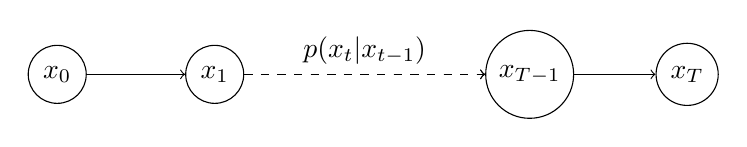
\begin{tikzpicture}
        % nodes
        \node (x0) [draw, circle] at (-4,0) {$x_0$};
        \node (x1) [draw, circle] at (-2,0) {$x_1$};
        \node (xT-1) [draw, circle] at (2,0) {$x_{T-1}$};
        \node (xT) [draw, circle] at (4,0) {$x_T$};

        % edges
        \draw[->] (x0) -- (x1);
        \draw[dashed, ->] (x1) -- (xT-1);
        \draw[->] (xT-1) -- (xT);

        % label
        \draw[dashed, ->] (x1) -- node[above] {$p(x_t|x_{t-1})$} (xT-1);
    \end{tikzpicture}
\end{center}
\vspace{0.5cm}

Such Markov chain is referred as the \textbf{forward diffusion process}, and $p(x_t|x_{t-1})$ is often referred as the \textbf{forward transition kernel}. Using the chain rule of probability and the Markov property, we can factorize the joint distribution of $x_0, \dots, x_T$ into:

$$
p(x_0, \dots, x_T) = p(x_0)\prod_{t=1}^Tp(x_t|x_{t-1})
$$

In practice, the most used forward process in continuous space is based on the injection of Gaussian noise:

$$
p(x_t|x_{t-1}) := \mathcal{N}(x_t;\sqrt{1-\beta_t}x_{t-1},\beta_tI)
$$

where $\beta_t \in (0,1)$ regulates the amount of noise that is injected at each step (the larger, the faster the convergence to the prior distribution). A useful property of the above process is that we can sample at any arbitrary time step in a closed form using the reparameterization trick. Given $\alpha_t := 1 - \beta_t,\bar{\alpha_t} := \prod_{i=1}^t\alpha_i$, and $\epsilon_t \sim \mathcal{N}(0,I)$ we have 

$$
\begin{array}{rl}
    x_t &= \sqrt{\alpha_t}x_{t-1} + \sqrt{1 - \alpha_t}\epsilon_{t-1} \\
    &= \sqrt{\alpha_t}(\sqrt{\alpha_{t-1}}x_{t-2} + \sqrt{1 - \alpha_{t-1}}\epsilon_{t-2}) + \sqrt{1 - \alpha_t}\epsilon_{t-1} \\
    &= \sqrt{\alpha_t\alpha_{t-1}}x_{t-2} + \sqrt{1 - \alpha_t\alpha_{t-1}}\hat{\epsilon}_{t-2} \\
    &= \dots \\
    &= \sqrt{\bar{\alpha_t}x_0} + \sqrt{1 - \bar{\alpha_t}}\hat{\epsilon}
\end{array}
$$

where $\epsilon_{t-2}$ and $\epsilon_{t-1}$ have been merged into $\hat{\epsilon}_{t-2}$.

Hence, we have 

$$
p(x_t|x_0) = \mathcal{N}(x_t;\sqrt{\bar{\alpha_t}}x_0,1-\bar{\alpha_t})
$$

This is also useful to show, as $\bar{\alpha_t} \to 0$, that 

$$
\lim_{t\to\infty}p(x_t|x_0) = \mathcal{N}(x_t;0,I)
$$

So for a sufficiently large $T$, $x_T \sim \mathcal{N}(0,I)$. In other words, this process ends up in corrupting the data into white noise.

\subsection*{Backward Process}

Now that we are able to gradually corrupt data points $x_0$ into noise, for generating new data samples we have to revert this process. We have seen that we can easily sample from $p(x_T)$, but sampling from 

$$
p(x_0, \dots, x_T) = p(x_T)\prod_{t=1}^Tp(x_{t-1}|x_t)
$$

is non-trivial, since we do not have access to the reverse transition kernels $p(x_{t-1}|x_t)^{*}$ that would allow us to perform ancestral sampling as in the forward process. Therefore, the reverse transition kernels $q_{\theta}(x_{t-1}|x_t)$, from which it is easy to sample and that can be easily computed, for example:

$$
q_{\theta}(x_{t-1}|x_t) := \mathcal{N}(x_{t-1};\mu_{\theta}(x_t,t),\Sigma_{\theta}(x_t,t))
$$

where the mean and covariance functions are neural networks. 

The objective is then to find parameters $\theta$ such that 

$$
q_{\theta}(x_0, \dots, x_T) := p(x_T)\prod_{t=1}^Tq_{\theta}(x_{t-1}|x_t) \approx p(x_0, \dots, x_T)
$$

\vspace{0.5cm}
\begin{center}
    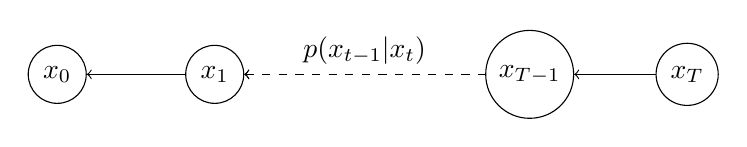
\begin{tikzpicture}
        % nodes
        \node (x0) [draw, circle] at (-4,0) {$x_0$};
        \node (x1) [draw, circle] at (-2,0) {$x_1$};
        \node (xT-1) [draw, circle] at (2,0) {$x_{T-1}$};
        \node (xT) [draw, circle] at (4,0) {$x_T$};

        % edges
        \draw[->] (x1) -- (x0);
        \draw[dashed, <-] (x1) -- (xT-1);
        \draw[->] (xT) -- (xT-1);

        % label
        \draw[dashed, <-] (x1) -- node[above] {$p(x_{t-1}|x_t)$} (xT-1);
    \end{tikzpicture}
\end{center}
\vspace{0.5cm}

The parametric kernels are learned by minimizing the Kullback-Leibler divergence between the forward and backward processes:

$$
\begin{array}{rl}
    D_{KL}(p(x_0,\dots,x_T)||q_{\theta}(x_0,\dots,x_T)) &= \mathbb{E}_{p(x_0,\dots,x_T)}\left[\log \frac{p(x_0,\dots,x_T)}{q_{\theta}(x_0,\dots,x_T)}\right] \\
    &= -\mathbb{E}_{p(x_0,\dots,x_T)}[\log q_{\theta}(x_0,\dots,x_T)] + \text{const} \\
    &= -\mathbb{E}_{p(x_0,\dots,x_T)}\left[\sum_{t=0}^T\log q_{\theta}(x_{t-1}|x_t)\right] + \text{const} 
\end{array}
$$

\textbf{Remark.} The forward process $p(x_0, \dots, x_T)$ was considered constant with respect to the parameters $\theta$. Although parameters of the forward process (as $\beta_t$) are usually considered fixed (hyperparameters), it is also possible to learn them. In that case we cannot consider the forward process as constant with respect to the parameters. 

Minimizing this inverse KL divergence is equivalent to solving a maximum likelihood estimation problem: we can sample full trajectories starting from sample from the dataset and use them to fit parametric functions $q_{\theta}$ by stochastic optimization, as in a supervised learning problem. 

\textbf{Remark.} It can be shown that, if forward transition kernels corrupts the data slowly enough ($T$ is large), then the reverse transition kernels will be approximately Gaussian. This is what makes the approximation of reverse transition kernels possible and approachable as a prediction problem. Conversely, if forward transition kernels add too much noise, the reverse transition probabilities can be multimodal, hence a parametric approximation would be intractable. 

\subsection*{Denoising parametrization}

There is empirical evidence that learning directly the backward transition kernels $q_\theta(x_{t-1}|x_t)$ is not the most effective strategy. Alternatively, it is possible to write the backward transition kernel in the following way:

$$
p(x_{t-1}|x_t) = \int_{x_0\in\mathcal{X}}p(x_{t-1}|x_0)\,dx_0 = \int_{x_0\in\mathcal{X}}p(x_{t-1}|x_t,x_0)p(x_0|x_t)\,dx_0
$$

This means that we can sample $x_{t-1}$ if we can sample $x_0 \sim p(x_0|x_t)$ and plug it into $p(x_{t-1}|x_t,x_0)$. It is possible to show that for the Gaussian diffusion process introduced above the distribution $p(x_{t-1}|x_t,x_0)$ is also a Gaussian and can be computed analytically:

$$
\begin{array}{c}
    p(x_{t-1}|x_t,x_0) = \mathcal{N}(x_{t-1};\mu_t(x_t, x_0), \sigma_tI) \\
    \mu_t(x_t,x_0) = \frac{\sqrt{\alpha_t}(1 - \bar{\alpha_{t-1}})}{1 - \bar{\alpha_t}}x_t + \frac{\sqrt{\bar{\alpha_{t-1}}\beta_t}}{1 - \bar{\alpha_t}}x_0 \\
    \sigma_t = \frac{(1 - \bar{\alpha}_{t-1})}{1 - \bar{\alpha_t}}\beta_t
\end{array}
$$

Instead $p(x_0|x_t)$ (the denoising kernel) has to be learned, again by fitting a parametric distribution $q_\theta(x_0|x_t)$. Interestingly, this works despite $p(x_0|x_t)$ being highly multimodal and non-Gaussian, so only a "mean" approximation is possible. 

However, it is common in DDPMs to avoid predicting directly $x_0$ given $x_t$. In fact, a model is trained to predict the noise that was added to $x_0$ in order to obtain $x_t$. Recall the property following from $p(x_t|x_0) = \mathcal{N}(x_t; \sqrt{\bar{\alpha_t}}x_0,1 - \bar{\alpha_t})$:

$$
x_t = \sqrt{\bar{\alpha_t}}x_0 + \sqrt{1 - \bar{\alpha_t}}\epsilon_t \text{ with }\epsilon_t \sim \mathcal{N}(0,I)
$$

We can rewrite the mean of $p(x_{t-1}|x_t,x_0)$, or $p(x_{t-1}|x_t,\epsilon_t)$, as 

$$
\mu_t(x_t,\epsilon_t) = \frac{1}{\sqrt{\alpha_t}}\left(x_t - \frac{1 - \alpha_t}{\sqrt{1 - \bar{\alpha_t}}}\epsilon_t\right)
$$

Now we can fit a parametric model $\epsilon_\theta(x_t,t)$ to approximate $p(\epsilon_t|x_t)$. This is usually done in a simplified way by minimizing the squared error:

$$
\begin{array}{rl}
    \mathcal{L}(\theta) &= \mathbb{E_{t,x_0,\epsilon_t}}[||\epsilon_t - \epsilon_\theta(x_t,t)||^2] \\
    &= \mathbb{E}_{t,x_0,\epsilon_t}\left[||\epsilon_t - \epsilon_\theta\left(\sqrt{\bar{\alpha_t}}x_0 + \sqrt{1 - \bar{\alpha_t}}\epsilon_t,t\right)||^2\right]
\end{array}
$$

where the time step $t$ is sampled uniformly in $\{1,\dots,T\}, x_0$ is randomly sampled from the dataset, and $\epsilon_t \sim \mathcal{N}(0,I)$. The training and sampling algorithm are then summarized as follows:
\begin{figure}[H]
    \centering
    \includegraphics[width=0.8\textwidth]{assets/fig51.png}
    \caption{Training and sampling algorithm for DDPMs}
    \label{fig:ddpm_algorithm}
\end{figure}

\textbf{Remark.} The empirical advantage of predicting the noise $\epsilon_t$ instead of $x_0$ could be due to the fact that it is easier to train a neural network when the target output is (marginally) distributed according to a normal distribution. 

\textbf{Summary}

A DDPM makes use of two Markov chains: a forward chain that perturbs data to noise, and a reverse chain that converts noise back to data. The forward Markov chain is designed with the goal to gradually transform any data distribution into a simple prior distribution (e.g., standard Gaussian). The backward Markov chain instead reverses the former starting from the known distribution and gradually converging to the data distribution. Since the backward Markov chain is unknown, it is learned by a deep neural network using examples generated with the forward process. New data points are subsequently generated by first sampling a random vector from the prior distribution, followed by ancestral sampling through the reverse Markov chain. 

\subsection*{Diffusion in discrete space}

Despite bein originally thought for data in continuous space, it is also possible to define a diffusion process in discrete space, even though its usefulness is questionable and subject of current research. Assuming without loss of generality data $x \in \{1,2,\dots,c\}^d$, there are two main kinds of discrete diffusion processes:
\begin{itemize}[label=$\blacktriangleright$, leftmargin=2em, itemindent=0em]
    \item \textbf{Uniform}: At each time step $t$, every component $x_t^i$ of $x_t$ switches to a random value with a given small probability $\epsilon_t$. The prior distribution of such diffusion process is the uniform over $\{1,2,\dots,c\}^d$.
    \item \textbf{Absorbing}: At each time step $t$, every component $x_t^i$ of $x_t$ switches to a partiular values called the "mask", often referred as the [MASK] token. The prior distribution of such diffusion process is the single point $[MASK]^d$, that is the absorbing state of the Markov chain. A variant of the absorbing diffusion process is when at each time step $t$ the $t^{th}$ component $x_t^t$ is masked. Modelling the corresponding reverse process is then equivalent to fitting an autoregressive model.
\end{itemize}

\subsection*{Score-based diffusion models}

Given the objective to sample from the distribution $p(x)$ that generated the data score-based models aim at estimating the so called \textit{score} of $p(x)$, defined as $\nabla_x\log p(x)$ and then use sampling techniques that exploit the knowledge of the score of the distribution. 

An example of score-based model is diffusion with stochstic differential equations (SDE), a generalization in continuous time of the Markov chain diffusion process discussed above, where the transition kernel $p(x_{t+\epsilon}|x_t)$ is implicitly defined through the following SDE:

$$
dx = f(x,t)\,dt + g(t)\,dw 
$$

where $\,dw \sim \mathcal{N}(0,I\,dt)$ is a Wiener process.

\begin{figure}[H]
    \centering
    \includegraphics[width=0.8\textwidth]{assets/fig52.png}
    \label{fig:diffusion_sde}
\end{figure}

Generation of new data points reduces to solving the inverse-time SDE, that it can be proven to be 

$$
\,dx = [f(x,t) - g^2(t)\nabla_x\log p_t(x)]\,dt + g(t)\,dw 
$$

FOr this we need to estimate the time dependent score $\nabla_x\log p_t(x)$, for example using a neural network $s_\theta(x,t)$. The most popular method is \textit{denoising score matching}, where the following loss is minimized:

$$
\mathbb{E}_{t\sim u(0,1),x_0\sim p(x_0),x_t\sim p(x_t|x_0)}||s_\theta(x_t,t) - \nabla_{x_t}\ln p(x_t|x_0)|| 
$$

that is deeply connected with the denoising loss of DDPMs.



